\documentclass[norsk, 12pt]{beamer}
% Add handout to documentclass options if wanted

\usepackage[latin1]{inputenc}
\usepackage[T1]{fontenc}
\usepackage{babel,textcomp}

\setlength{\arrayrulewidth}{1.6pt}
\renewcommand{\arraystretch}{1.2}
\newlength{\Tcalc}

\usepackage[T1]{fontenc}
\usepackage{graphicx}
\usepackage{amsmath}
\usepackage{amssymb}
\usepackage{amsbsy}
\usepackage{amsfonts}
\usepackage{color}
\usepackage{xcolor}
\usepackage{epstopdf}
\usepackage{fancyvrb}
\usepackage{parskip}
\usepackage{url}
\usepackage{listings}

\definecolor{javared}{rgb}{0.6,0,0} % for strings
\definecolor{javagreen}{rgb}{0.25,0.5,0.35} % comments
\definecolor{javapurple}{rgb}{0.5,0,0.35} % keywords
\definecolor{javadocblue}{rgb}{0.25,0.35,0.75} % javadoc

\lstset{language=Matlab,
basicstyle=\ttfamily
keywordstyle=\color{javapurple},%\bfseries,
stringstyle=\color{javared},
commentstyle=\color{javagreen},
morecomment=[s][\color{javadocblue}]{/**}{*/},
morekeywords={super, with},
% numbers=left,
% numberstyle=\tiny\color{black},
stepnumber=2,
numbersep=10pt,
tabsize=2,
showspaces=false,
% captionpos=b,
showstringspaces=false,
frame=  false,
breaklines=true}

\setbeamertemplate{frametitle}
{\begin{centering}\smallskip
\insertframetitle\par
\smallskip\end{centering}}
\setbeamertemplate{itemize item}{$\bullet$}
\setbeamertemplate{navigation symbols}{}
\setbeamertemplate{footline}[text line]{%
\hfill\strut{%
\scriptsize\sf\color{black!60}%
\quad\insertframenumber
   }%
    \hfill
}

% Define some colors:
\definecolor{DarkFern}{HTML}{407428}
\definecolor{DarkCharcoal}{HTML}{4D4944}
\colorlet{Fern}{DarkFern!85!white}
\colorlet{Charcoal}{DarkCharcoal!85!white}
\colorlet{LightCharcoal}{Charcoal!50!white}
\colorlet{AlertColor}{orange!80!black}
\colorlet{DarkRed}{red!70!black}
\colorlet{LightBlue}{blue!70!white}
\colorlet{DarkBlue}{blue!70!black}
\colorlet{DarkGreen}{green!70!black}

% Use the colors:
\setbeamercolor{title}{fg=Fern}
\setbeamercolor{frametitle}{fg=Fern}
\setbeamercolor{normal text}{fg=Charcoal}
\setbeamercolor{block title}{fg=black,bg=Fern!25!white}
\setbeamercolor{block body}{fg=black,bg=Fern!25!white}
\setbeamercolor{alerted text}{fg=AlertColor}
\setbeamercolor{itemize item}{fg=Charcoal}

\newcommand{\frn}[1]{\textcolor{Fern}{#1}}
\newcommand{\alrt}{\color{AlertColor}}
\newcommand{\bt}[1]{\textbf{#1}}
\newcommand{\kommando}[1]{\textcolor{AlertColor}{\texttt{\textbackslash #1}}}
\newcommand{\ds}{\displaystyle}

\title{Studies of near-gaussian beams}
\author{Jonas van den Brink}
\institute{}
\date{1. desember 2014}

\setbeamertemplate{frametitle}{\vspace{0.5cm} \insertframetitle} 

\begin{document}
\pagestyle{empty}

\section{Introduksjon}

\begin{frame}[fragile]
\begin{center}	
{\Huge \color{DarkFern} Computational cardiac electrophyisology}
\begin{center}
\vspace{0.1cm}
\includegraphics[width=0.7\textwidth]{snapshot3.png}
\vspace{0.1cm}
\end{center}
{\centering \color{Charcoal} Jonas van den Brink}
\end{center}
\end{frame}

\begin{frame}[fragile]
\frametitle{Computational cardiology is a problem in multiscale modeling}
\begin{center}
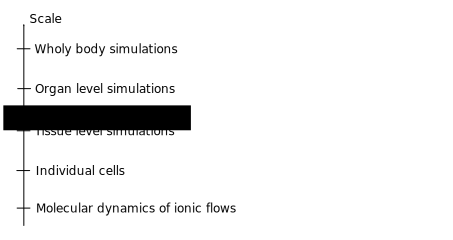
\includegraphics[width=\textwidth]{multiscale0.pdf}
\end{center}
\end{frame}

\begin{frame}[fragile]
\frametitle{Computational cardiology is a problem in multiscale modeling}
\begin{center}
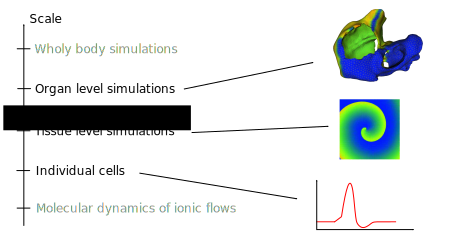
\includegraphics[width=\textwidth]{multiscale1.pdf}
\end{center}
\end{frame}


\begin{frame}[fragile]
\frametitle{Differences in ionic concentration lead to an electric charge difference}
\begin{center}
\includegraphics[width=\textwidth]{membrane0.pdf}
\end{center}
\end{frame}

\begin{frame}[fragile]
\frametitle{Differences in ionic concentration lead to an electric charge difference}
\begin{center}
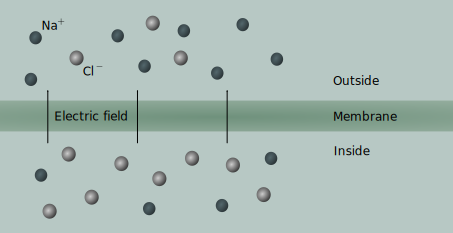
\includegraphics[width=\textwidth]{membrane1.pdf}
\end{center}
\end{frame}

\begin{frame}[fragile]
\frametitle{Heart cells are excitable}
\begin{center}
\includegraphics[width=\textwidth]{ap0.pdf}
\end{center}
\end{frame}

\begin{frame}[fragile]
\frametitle{Heart cells are excitable}
\begin{center}
\includegraphics[width=\textwidth]{ap1.pdf}
\end{center}
\end{frame}

\begin{frame}[fragile]
\frametitle{Heart cells are excitable}
\begin{center}
\includegraphics[width=\textwidth]{ap2.pdf}
\end{center}
\end{frame}

\begin{frame}[fragile]
\frametitle{Heart cells are excitable}
\begin{center}
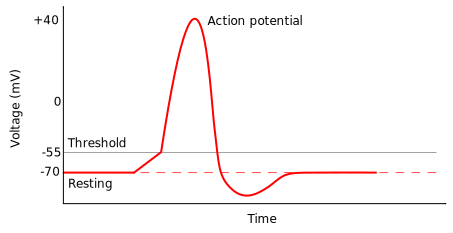
\includegraphics[width=\textwidth]{ap3.pdf}
\end{center}
\end{frame}

\begin{frame}[fragile]
\frametitle{Heart cells are excitable}
\begin{center}
\includegraphics[width=\textwidth]{ap4.pdf}
\end{center}
\end{frame}

\begin{frame}[fragile]
\begin{center}
\includegraphics[width=\textwidth]{ap5.jpeg}
\end{center}
\end{frame}

\begin{frame}[fragile]
\frametitle{Why do cells fire?}
\end{frame}


\begin{frame}[fragile]
\frametitle{Why do cells fire?}
\begin{center}
	\includegraphics[width=\textwidth]{HH0}
\end{center}
\end{frame}

\begin{frame}[fragile]
\frametitle{Why do cells fire?}
\begin{center}
	\includegraphics[width=\textwidth]{HH1}
\end{center}
\end{frame}

\begin{frame}[fragile]
\frametitle{We can use Hodgekin-Huxley models to describe excitable cells}

\begin{center}
	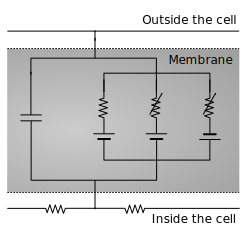
\includegraphics[width=0.5\textwidth]{HH2}
\end{center}

Leads to a set of highly non-linear ODEs.

There are an extreme amount of different cell models in the litterature.
\end{frame}


\begin{frame}[fragile]
\frametitle{A cell firing will affect nearby cells as the charge literally diffuses between cells}
\begin{center}
	\includegraphics[width=0.8\textwidth]{matches}
\end{center}
This is an example of a reaction-diffusion phenomenon.
\end{frame}

\begin{frame}[fragile]
\frametitle{The reaction-diffusion leads to a wavefront propagating through the tissue}
\begin{center}
	\includegraphics[width=0.8\textwidth]{fire}
\end{center}
\end{frame}

\begin{frame}[fragile]
\frametitle{We can use operator splitting to seperate the reaction-diffusion equation}
\begin{center}
\includegraphics[width=\textwidth]{op_split0.pdf}
\end{center}
\end{frame}

\begin{frame}[fragile]
\frametitle{We can use operator splitting to seperate the reaction-diffusion equation}
\begin{center}
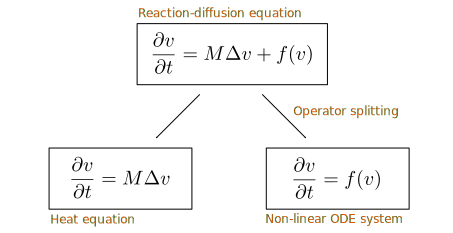
\includegraphics[width=\textwidth]{op_split1.pdf}
\end{center}
\end{frame}


\begin{frame}[fragile]
\frametitle{We then solve the equations in a 2D or 3D mesh}
\begin{center}
\includegraphics[width=\textwidth]{snapshot0}
\end{center}

\visible<2->{
[Movie]
}
\end{frame}


\begin{frame}[fragile]
\frametitle{}
\begin{center}
\includegraphics[width=\textwidth]{ecg0}
\end{center}
\end{frame}

\begin{frame}[fragile]
\frametitle{}
\begin{center}
\includegraphics[width=\textwidth]{ecg1}
\end{center}
\end{frame}

\begin{frame}[fragile]
\frametitle{}
\begin{center}
\includegraphics[width=\textwidth]{ecg2}
\end{center}
\end{frame}

\begin{frame}[fragile]
\frametitle{}
\begin{center}
\includegraphics[width=\textwidth]{ecg3}
\end{center}
\end{frame}

\begin{frame}[fragile]
\frametitle{}
\begin{center}
\includegraphics[width=\textwidth]{ecg4}
\end{center}
\end{frame}

\begin{frame}[fragile]
\frametitle{}
\begin{center}
\includegraphics[width=\textwidth]{ecg5}
\end{center}
\end{frame}

\begin{frame}[fragile]
\frametitle{During a heart cycle, the heart depolarizes and becomes an electric dipole}

An electrocardiogram (EKG) measures the dipole field 
\begin{center}
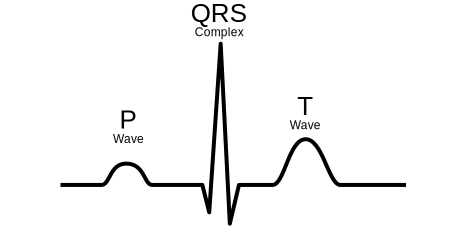
\includegraphics[width=\textwidth]{pqrst}
\end{center}
\end{frame}

\begin{frame}[fragile]
\frametitle{Fibrillation is rapid, unscynchronized contraction of muscle cell}

It is often caused by reentrant waves
\begin{center}
\includegraphics[width=\textwidth]{ecgr}
\end{center}
These waves never die out and so the heart doesn't contract as one.

\visible<2->{
[Movie] + [Gifs]
}
\end{frame}


\begin{frame}[fragile]
\frametitle{Ventricular fibrillation is always deadly, but atrial fibrillation is not}

\visible<2->{
The Maze procedure is a surgical treatment of atrial fibrillation
}

\vspace{1cm}

\visible<3->{
Ablation is a therapy where parts of the atria are burnt
}

\vspace{1cm}

\visible<4->{
The causes of atrial fibrillation and these procedures are not well understood
}
\end{frame}

\begin{frame}[fragile]
\begin{center}
\includegraphics[width=\textwidth]{relapse}
\end{center}
\end{frame}

\begin{frame}[fragile]
\frametitle{Patient-specific modelling can make treatments of atrial fibrillation more effective}

Cardiac modelling is one of the most important tools in developing new treatment for heart conditions such as atrial fibrillation

\vspace{1cm}

\visible<2-> {
By using measurements from ECG, MRI and similar, our simulations can be adapted on a patient-by-patient basis.
}
\end{frame}

\begin{frame}[fragile]
\frametitle{Computational Physiology (INF5560) gives a good introduction to cardiac modelling}

\begin{center}
\includegraphics[width=\textwidth]{GroupBear-2}	
\end{center}
\end{frame}


\end{document}